\chapter{TBD}\label{ch:undefined}
En este capítulo desarrollamos el marco de trabajo realizado, las decisiones tomadas en la selección de determinados métodos expuesto en el capítulo anterior, las  herramientas utilizadas y el tipo de arquitectura seleccionada para la extracción de los datos.

\section{Pipeline}\label{sec: pipeline}
En \ac{ml} un \textit{pipeline} es el flujo de trabajo en el cual se desarrollaran las tareas, esto nos permite automatizar los datos y el flujo de tareas. Un pipeline consiste en diversos pasos donde cada uno de ellos implica determinada tarea como se menciono previamente, los pipeline son generalmente iterativos.
%https://hackernoon.com/machine-learning-model-pipelines-part-i-e138b7a7c1ef

La construcción de pipelines proporciona muchas ventaja al igual que un desarrollo de software tradicional; estas ventajas incluyen:
\begin{itemize}
\item \textbf{Flexibilidad}: Cada unidad, tareas, son fáciles de reemplazar de modo que si se quiere cambiar la implementación de determinada tarea se lo puede realizar sin afectar el resto del sistema.

\item \textbf{Extensibilidad}: A partir de que el sistema esta dividido se puede extender nuevas unidades, es decir, agregar nuevos pasos al flujo de trabajo de manera transparente sin afectar el correcto funcionamiento del flujo de trabajo.

\item \textbf{Legibilidad}: Al ser cada tarea atómica nos permite lograr una mejor compresión de cada una de las unidades/pasos que se desarrollaron ayudando a identificar posibles errores.

\end{itemize}

En la siguiente imagen\ref{Fig:pipeline} podemos ver un pipeline de desarrollo en aprendizaje supervisado:

\begin{figure}[H] \centering
  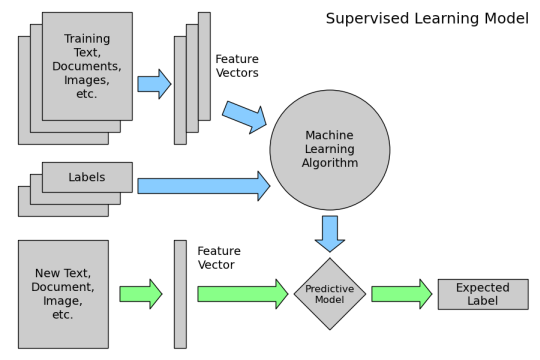
\includegraphics[height=8cm,keepaspectratio=true,clip=true]{imagenes/tbd/pipeline-sp.png}
  \caption{Pipeline}\label{Fig:pipeline}
\end{figure}

Partiendo de la figura anterior, se adapto el pipeline de acuerdo a las necesidades del trabajo de la siguiente manera:

\begin{figure}[H] \centering
  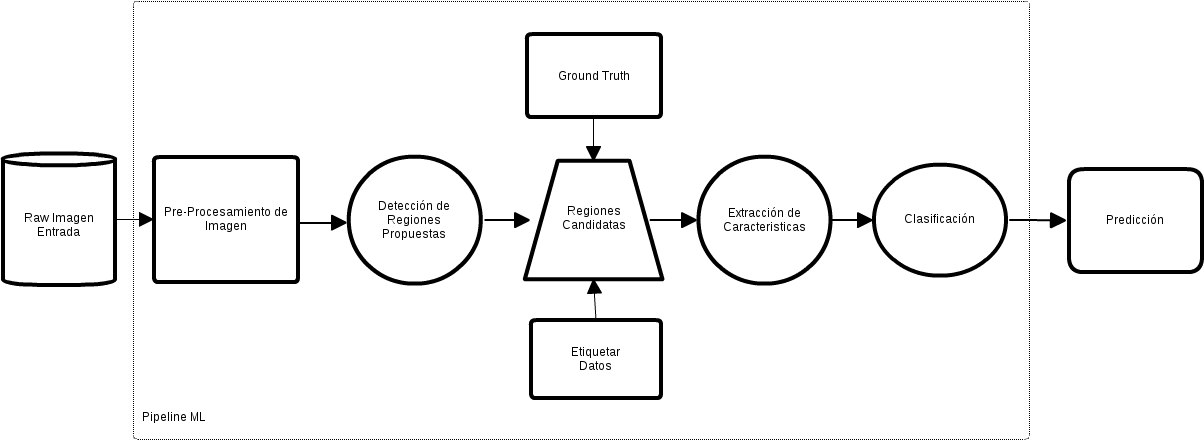
\includegraphics[height=5cm,keepaspectratio=true,clip=true]{imagenes/tbd/pipeline.png}
  \caption{Pipeline de Trabajo}\label{Fig:pipeline-mio}
\end{figure}

%https://www.datanami.com/2018/09/05/how-to-build-a-better-machine-learning-pipeline/
\subsection{Descripción del Pipeline desarrollado}\label{sub:desc-pipeline}

\subsubsection*{Imágenes Raw}
Este bloque hace referencia a las imágenes raw, crudas, obtenidas a través de la pagina de \ac{conae} como se menciona en el capítulo \ref{ch:recopilacion}. Estas imágenes están codificadas en un formato "h5" por cada una de las bandas del sensor.

\subsubsection*{Pre-procesamiento}
En este paso del pipeline de trabajo se realizo un procesamiento de las imágenes raw obtenidas a partir del item anterior. Este procesamiento incluye la conversión de los datos raw a imágenes con diferentes combinaciones de bandas utilizando para esto la herramienta ENVI para la realización de este trabajo\ref{sec:envi}.	

\begin{figure}[H] \centering
  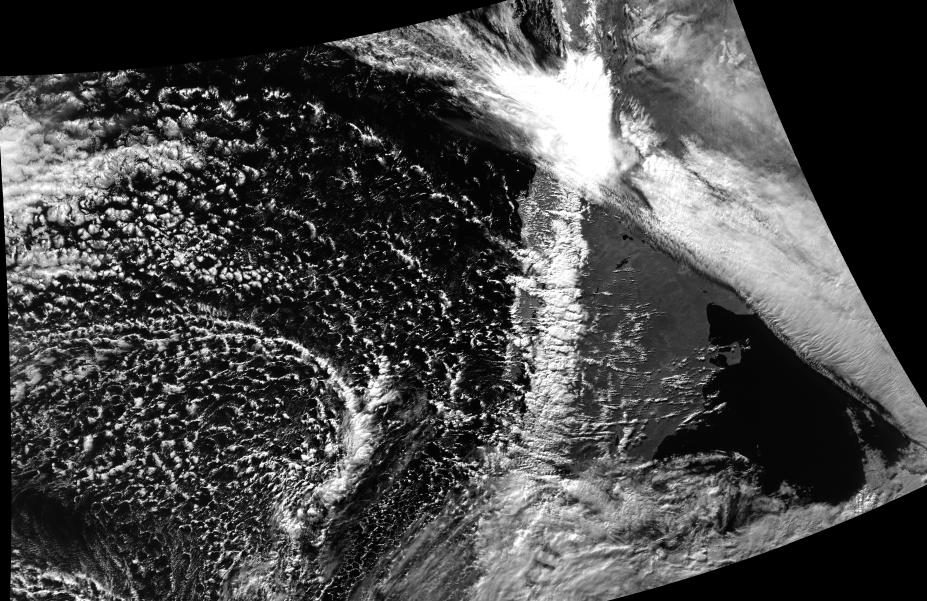
\includegraphics[height=7cm,keepaspectratio=true,clip=true]{imagenes/tbd/pre-img.png}
  \caption{Imagen final obtenida luego del procesamiento.}\label{Fig:img-final}
\end{figure}

\subsubsection*{Detección de regiones propuesta}
Luego de la conversión de datos raw a imágenes, se evaluaron que métodos de detección de regiones candidatas usar \ref{sec:regionespropuestas}.

Las siguientes consideraciones tomadas a la hora de elegir determinadas metodologías fueron:
\begin{table}[H]
\centering
\begin{tabular}{|p{2cm}|p{6cm}|p{8cm}|}
    \hline 
     & \centering \textbf{Ventajas} & \multicolumn{1}{c|}{\centering \textbf{Desventajas}} \\
    \hline
    \centering Selective Search & \parbox[p][0.2\textwidth][c]{6cm}{
    \begin{itemize}
        \item Fácil implementación en python	
    \end{itemize}}  &  \parbox[p][0.2\textwidth][c]{7.5cm}{
    \begin{itemize}
        \item Tiempo de ejecución muy alto para imágenes de resolución mayores; ejemplo: 2800x3000px.	
    \end{itemize} } \\ \hline
    \centering Edges Boxes & \parbox[p][0.2\textwidth][c]{6cm}{
    \begin{itemize}
        \item Buen tiempo de ejecución con imágenes de gran tamaño
        \item Reconocimientos de regiones de menor tamaño
    \end{itemize} } & \parbox[p][0.2\textwidth][c]{7.5cm}{
    \begin{itemize}
        \item No se encontró una implementación optima en python.	
    \end{itemize} } \\ \hline 
     \centering BING & \parbox[p][0.2\textwidth][c]{6cm}{
    \begin{itemize}
        \item El tiempo de ejecución en imágenes de gran tamaño es optimo
    \end{itemize} } &  \parbox[p][0.2\textwidth][c]{7.5cm}{
    \begin{itemize}
        \item Baja probabilidad de encontrar regiones de menor tamaño en imágenes grandes.
    \end{itemize} } \\ \hline
\end{tabular}
\caption{Análisis de métodos Regiones Propuestas}
\label{tabla:comparacionregiones}
\end{table}

El método utilizado para la extracción de regiones candidatas fue \textit{Selective search}

\subsubsection*{Regiones candidatas}
Esta etapa del pipeline, ya con las regiones candidatas obtenidas en el punto anterior aplicamos lo que en el marco teórico se desarrollo como \ac{nms} \ref{sec:nms}. Aplicando esta técnica descartamos regiones quedándonos con aquellas que cumplen determinado criterio de solapamiento.

Para finalizar se recorto la imagen por cada regiones candidatas obtenidas; a su ves se calculo si cada región candidata se solapaba con algunos de los \textit{graund truth} etiquetados previamente en la imagen \ref{sec:grodunthruh}, almacenando con los valores 0 si no existía solapamiento entre regiones candidatas y 1 en caso contrario.

\subsubsection*{Extracción de características}
En esta paso del pipeline se utilizo una red neuronal pre entrenada llamada \textit{Resnet50}\ref{sec:arquitecturasdered}. Obteniendo por cada región un vector de 2048 elementos que la representa.

Estos datos se almacenaron en un archivo \textit{.mat} para poder luego ser utilizado en el paso de clasificación.

\subsubsection*{Clasificación}
El proceso de clasificación podríamos decir que es el ultimo paso importante del pipeline desarrollado, en el a partir de los datos etiquetados junto con sus vectores de característica correspondiente se entreno un clasificador linear realizando cross validation en cada etapa, para luego obtener métricas mencionadas en \ref{sec:metricas} que seran las que nos indiquen que tan bien generaliza nuestro modelo.

\subsubsection*{Predicción}
La ultima etapa del pipeline es la predicción en esta etapa a partir del modelo entrenado en el item anterior vamos a tratar de predecir una imagen nueva que nunca vio el modelo. Para poder realizar este paso la nueva imagen debe pasar todos los pasos descripto en el pipeline excluyendo el etiquetado y en entrenamiento de clasificación.



Un pipeline en \ac{ml} es un proceso iterativo; en este trabajo se realizo diversas iteraciones tanto a nivel individual de cada paso como a nivel global. 